% Ephemeral Bump Arena for a Bytecode Virtual Machine: Design and Memory Safety Proof
%
% Compile with: pdflatex lattice_arena_safety.tex
%
\documentclass[11pt]{article}

\usepackage[margin=1in]{geometry}
\usepackage{amsmath,amssymb,amsthm}
\usepackage{mathpartir}
\usepackage{stmaryrd}        % \llbracket, \rrbracket
\usepackage{xcolor}
\usepackage{microtype}
\usepackage{enumitem}
\usepackage{booktabs}
\usepackage{listings}
\usepackage{tikz}
\usepackage{needspace}
\usepackage{hyperref}

\usetikzlibrary{arrows.meta, positioning, fit, backgrounds, calc, decorations.pathreplacing}

% ── Theorem environments ──
\newtheorem{theorem}{Theorem}[section]
\newtheorem{lemma}[theorem]{Lemma}
\newtheorem{proposition}[theorem]{Proposition}
\newtheorem{corollary}[theorem]{Corollary}
\newtheorem{definition}[theorem]{Definition}
\newtheorem{remark}[theorem]{Remark}

% ── Notation macros ──
\newcommand{\kw}[1]{\mathbf{#1}}           % keyword
\newcommand{\flx}{\kw{flux}}
\newcommand{\fixkw}{\kw{fix}}
\newcommand{\letkw}{\kw{let}}
\newcommand{\freezekw}{\kw{freeze}}
\newcommand{\thawkw}{\kw{thaw}}
\newcommand{\clonekw}{\kw{clone}}
\newcommand{\returnkw}{\kw{return}}
\newcommand{\spawnkw}{\kw{spawn}}

% Phase tags
\newcommand{\fluid}{\mathsf{fluid}}
\newcommand{\crystal}{\mathsf{crystal}}
\newcommand{\unphased}{\bot}

% Phase set
\newcommand{\Phase}{\mathsf{Phase}}

% Semantic domains
\newcommand{\Val}{\mathsf{Val}}
\newcommand{\TVal}{\mathsf{TVal}}
\newcommand{\Env}{\mathsf{Env}}
\newcommand{\Store}{\mathsf{Store}}
\newcommand{\Loc}{\mathsf{Loc}}
\newcommand{\Region}{\mathsf{Region}}
\newcommand{\RegId}{\mathsf{RId}}
\newcommand{\FHeap}{\mathsf{FHeap}}
\newcommand{\RStore}{\mathsf{RStore}}
\newcommand{\Arena}{\mathsf{Arena}}
\newcommand{\Page}{\mathsf{Page}}
\newcommand{\Expr}{\mathsf{Expr}}
\newcommand{\Stmt}{\mathsf{Stmt}}
\newcommand{\Decl}{\mathsf{Decl}}
\newcommand{\Var}{\mathsf{Var}}

% Arena-specific notation
\newcommand{\Stack}{\mathsf{Stack}}
\newcommand{\Frames}{\mathsf{Frames}}
\newcommand{\Globals}{\mathsf{Globals}}
\newcommand{\Upvals}{\mathsf{Upvals}}
\newcommand{\ephemeral}{\mathsf{ephemeral}}
\newcommand{\rnone}{\mathsf{REGION\_NONE}}
\newcommand{\reph}{\mathsf{REGION\_EPHEMERAL}}
\newcommand{\promote}{\mathsf{promote}}
\newcommand{\dc}[1]{\mathsf{deepclone}(#1)}
\newcommand{\resetarena}{\mathsf{reset}}
\newcommand{\reachable}{\mathcal{R}}
\newcommand{\opcode}[1]{\texttt{OP\_#1}}

% Tagged value notation: v^σ
\newcommand{\tval}[2]{#1^{#2}}

% ── Listings configuration ──
\lstdefinelanguage{Lattice}{
  morekeywords={fn,let,flux,fix,struct,if,else,for,in,while,return,freeze,thaw,clone,forge,true,false,print,spawn},
  sensitive=true,
  morecomment=[l]{//},
  morecomment=[s]{/*}{*/},
  morestring=[b]",
  literate={->}{$\rightarrow$}{2},
}
\lstset{
  language=Lattice,
  basicstyle=\small\ttfamily,
  keywordstyle=\bfseries,
  commentstyle=\itshape\color{gray},
  stringstyle=\color{darkgray},
  numbers=left,
  numberstyle=\tiny\color{gray},
  numbersep=5pt,
  frame=single,
  framesep=3pt,
  xleftmargin=1.5em,
  breaklines=true,
  captionpos=b,
  aboveskip=0.8\baselineskip,
  belowskip=0.5\baselineskip,
}

% ── Document ──
\title{\textbf{Ephemeral Bump Arena for a Bytecode Virtual Machine:\\Design and Memory Safety Proof}}
\author{Alex Jokela\\{\small\texttt{alex.c.jokela@gmail.com}}}
\date{February 2026}

\begin{document}
\maketitle
\thispagestyle{empty}

\begin{abstract}
Per-allocation overhead from \texttt{malloc}/\texttt{free} is a significant cost
in bytecode virtual machines for dynamically-typed languages, particularly for
short-lived string temporaries produced by concatenation and interpolation.
We present an \emph{ephemeral bump arena} that allocates these temporaries with
$O(1)$ bump-pointer allocation and reclaims them in bulk at statement boundaries
via $O(\text{pages})$ reset.  The key challenge is ensuring that no dangling
pointers survive arena resets: any value that escapes the expression-temporary
lifetime must be \emph{promoted} to heap-allocated storage before the arena is
recycled.  We formalize the \emph{Arena Safety Invariant}---that no reachable
value references ephemeral memory at the point of reset---and prove it correct
by exhaustive case analysis over all escape paths in the Lattice bytecode VM.
The proof is validated empirically by a 815-test suite passing under
AddressSanitizer.
\end{abstract}

%% ════════════════════════════════════════════════════════════════════
\section{Introduction}
\label{sec:intro}

The Lattice programming language is a dynamically-typed language with first-class
immutability semantics (a \emph{phase system}), rich string operations, and a
bytecode virtual machine for execution.  String concatenation and interpolation
are pervasive operations---every \texttt{print} call with formatted output, every
loop building a result string, and every string comparison chain produces
temporary string values that are consumed within a single expression and then
discarded.

In a na\"ive implementation, each temporary string requires a \texttt{malloc}
call for creation and a \texttt{free} call for deallocation.  For a chain of $N$
concatenations (e.g., \lstinline|a + b + c + d|), this produces $N-1$
intermediate strings, each requiring a separate allocation and deallocation.  The
per-allocation overhead---including allocator metadata, fragmentation, and system
call costs---dominates the actual string copying work.

We address this with an \emph{ephemeral bump arena}: a page-based arena allocator
that serves all string temporaries within a statement, then resets in bulk at the
statement boundary.  Bump allocation is $O(1)$ (a pointer increment with
alignment), and reset is $O(\text{pages})$ (resetting the \texttt{used} counter
on each page in the chain).

The critical correctness challenge is that some expression results \emph{escape}
the statement lifetime: they may be assigned to local variables, stored in global
bindings, captured in closures, or inserted into compound data structures.  If
such an escaping value still points into the arena when it is reset, the result
is a dangling pointer and undefined behavior.  We solve this with a
\emph{promotion} strategy: at every point where a value can escape to long-lived
storage, we deep-clone ephemeral values to \texttt{malloc}-backed memory.

This paper makes the following contributions:
\begin{enumerate}[nosep]
  \item The design of an ephemeral bump arena integrated into a stack-based
        bytecode VM (\S\ref{sec:design}).
  \item A taxonomy of all escape points where values transition from
        expression-temporary to long-lived storage (\S\ref{sec:escape}).
  \item A formal proof of the Arena Safety Invariant---that no reachable value
        holds ephemeral memory at reset time (\S\ref{sec:proof}).
  \item A case study of a soundness bug that escaped both a 815-test suite and
        AddressSanitizer, motivating the need for formal reasoning
        (\S\ref{sec:bug}).
  \item Empirical validation with AddressSanitizer and targeted escape-path
        tests (\S\ref{sec:empirical}).
\end{enumerate}

%% ════════════════════════════════════════════════════════════════════
\section{Background}
\label{sec:background}

\subsection{The Lattice VM}
\label{sec:vm}

Lattice programs are compiled to bytecode and executed by a stack-based virtual
machine.  The VM maintains a value stack, a call-frame stack, a global
environment, and a set of heap-allocated upvalues for closures.  Every runtime
value is represented as a \texttt{LatValue} struct carrying a type tag, a phase
tag ($\fluid$, $\crystal$, or $\unphased$), a \emph{region identifier}, and a
payload union.

The region identifier classifies the memory backing a value's heap data:
\begin{itemize}[nosep]
  \item $\rnone$ ($(size\_t){-1}$): the value's string/array/struct data was
        allocated with \texttt{malloc} and is owned normally.
  \item $\reph$ ($(size\_t){-2}$): the value's data resides in the ephemeral
        bump arena.
  \item A numeric crystal region ID: the value was frozen into an arena-based
        crystal region.
\end{itemize}

\subsection{Value Lifecycle}
\label{sec:lifecycle}

A value in the Lattice VM follows a well-defined lifecycle:
\begin{enumerate}[nosep]
  \item \textbf{Creation}: produced by a bytecode instruction (literal load,
        arithmetic, string concat, container construction).
  \item \textbf{Stack residence}: pushed onto the value stack as an expression
        temporary.
  \item \textbf{Escape}: optionally moves to long-lived storage (local binding,
        global, upvalue, container element, return value).
  \item \textbf{Deallocation}: freed when the owning scope exits, the container
        is freed, or the arena is reset.
\end{enumerate}

The ephemeral arena is relevant at steps 1--3: values created in the arena
(step~1) reside on the stack (step~2) and must be promoted before the arena
resets if they escape (step~3).

\subsection{Notation}
\label{sec:notation}

We model the VM state as a tuple $\mathcal{V} = (S, G, F, U, A)$ where:
\begin{itemize}[nosep]
  \item $S : \Stack$ is the value stack, an ordered sequence of \texttt{LatValue}s.
  \item $G : \Globals$ is the global environment, mapping names to values.
  \item $F : \Frames$ is the call-frame stack, each frame referencing a slice of $S$.
  \item $U : \Upvals$ is the set of open and closed upvalues.
  \item $A : \Arena$ is the ephemeral bump arena.
\end{itemize}

We write $v.\mathit{rid}$ for the region identifier of value $v$, and
$v.\mathit{rid} = \reph$ to indicate that $v$'s heap data resides in~$A$.

%% ════════════════════════════════════════════════════════════════════
\section{Ephemeral Bump Arena Design}
\label{sec:design}

\subsection{Data Structure}
\label{sec:data-structure}

The bump arena (\texttt{BumpArena}) is a linked list of fixed-size pages
(4096~bytes each), with a current-page pointer and a bump offset:

\begin{lstlisting}[language=C,title={\texttt{include/memory.h}}]
typedef struct BumpArena {
    ArenaPage  *pages;       // current page pointer
    ArenaPage  *first_page;  // head of chain (kept across resets)
    size_t      total_bytes;
} BumpArena;
\end{lstlisting}

Allocation is a pointer bump with 8-byte alignment:

\[
  \texttt{bump\_alloc}(A, n) =
  \begin{cases}
    A.\mathit{pages}.\mathit{data} + A.\mathit{pages}.\mathit{used}
      & \text{if } A.\mathit{pages}.\mathit{used} + \lceil n \rceil_8 \le A.\mathit{pages}.\mathit{cap} \\
    \text{advance to next page or allocate new page}
      & \text{otherwise}
  \end{cases}
\]

where $\lceil n \rceil_8 = (n + 7) \mathbin{\&} \mathord{\sim}7$ is 8-byte alignment.

\subsection{Region Tagging}
\label{sec:tagging}

Every \texttt{LatValue} carries a \texttt{region\_id} field that classifies its
memory ownership:

\begin{center}
\begin{tabular}{lll}
\toprule
\textbf{Sentinel} & \textbf{Value} & \textbf{Meaning} \\
\midrule
\texttt{REGION\_NONE}      & $(size\_t){-1}$ & Normal \texttt{malloc} ownership \\
\texttt{REGION\_EPHEMERAL} & $(size\_t){-2}$ & Ephemeral arena allocation \\
Numeric ID                  & $0, 1, 2, \ldots$ & Crystal region (frozen data) \\
\bottomrule
\end{tabular}
\end{center}

The \texttt{value\_free} function checks \texttt{region\_id}: values with
$\mathit{rid} \ne \rnone$ are skipped (their memory is managed by
the arena or region system, not individually freed).

\subsection{Ephemeral Value Creation}
\label{sec:creation}

Only two opcodes produce ephemeral values:
\begin{enumerate}[nosep]
  \item \opcode{ADD} (when both operands are strings): concatenates strings and
        allocates the result in the arena via \texttt{vm\_ephemeral\_string}.
  \item \opcode{CONCAT} (string interpolation): builds the interpolated string
        in the arena.
\end{enumerate}

\needspace{14\baselineskip}
The helper function \texttt{vm\_ephemeral\_string} takes a \texttt{malloc}'d
string, copies it into the arena via \texttt{bump\_strdup}, frees the original,
and returns a \texttt{LatValue} with $\mathit{rid} = \reph$:

\begin{lstlisting}[language=C,title={\texttt{src/vm.c}: Ephemeral string creation}]
static inline LatValue vm_ephemeral_string(VM *vm, char *s) {
    if (vm->ephemeral) {
        char *arena_str = bump_strdup(vm->ephemeral, s);
        free(s);
        LatValue v;
        v.type = VAL_STR;
        v.phase = VTAG_UNPHASED;
        v.region_id = REGION_EPHEMERAL;
        v.as.str_val = arena_str;
        return v;
    }
    return value_string_owned(s);
}
\end{lstlisting}

\subsection{Statement-Boundary Reset}
\label{sec:reset}

The compiler emits \opcode{RESET\_EPHEMERAL} at statement boundaries.  When
executed, the VM first promotes all ephemeral values on the stack, then resets
the arena:

\begin{lstlisting}[language=C,title={\texttt{src/vm.c}: Arena reset with stack scan}]
case OP_RESET_EPHEMERAL: {
    for (LatValue *slot = vm->stack; slot < vm->stack_top; slot++)
        vm_promote_value(slot);
    bump_arena_reset(vm->ephemeral);
    break;
}
\end{lstlisting}

The \texttt{bump\_arena\_reset} function iterates through the page chain and
resets each page's \texttt{used} counter to zero, then repoints the current-page
pointer to the first page.  The page chain itself is retained for reuse.

\begin{figure}[h]
\centering
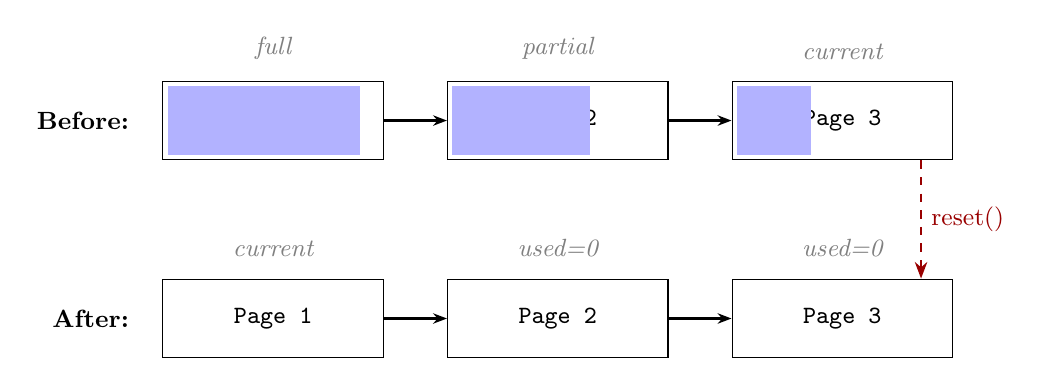
\begin{tikzpicture}[
    page/.style={draw, minimum width=2.8cm, minimum height=1cm, font=\small\ttfamily},
    arrow/.style={-{Stealth[length=5pt]}, thick},
    label/.style={font=\small\itshape, text=gray}
]
  % Pages
  \node[page] (p1) {Page 1};
  \node[page, right=0.8cm of p1] (p2) {Page 2};
  \node[page, right=0.8cm of p2] (p3) {Page 3};

  % Arrows between pages
  \draw[arrow] (p1) -- (p2);
  \draw[arrow] (p2) -- (p3);

  % Used indicators (before reset)
  \fill[blue!30] ([xshift=2pt,yshift=2pt]p1.south west) rectangle ([xshift=-0.3cm,yshift=-2pt]p1.north east);
  \fill[blue!30] ([xshift=2pt,yshift=2pt]p2.south west) rectangle ([xshift=-1.0cm,yshift=-2pt]p2.north east);
  \fill[blue!30] ([xshift=2pt,yshift=2pt]p3.south west) rectangle ([xshift=-1.8cm,yshift=-2pt]p3.north east);

  % Labels
  \node[label, above=0.15cm of p1] {full};
  \node[label, above=0.15cm of p2] {partial};
  \node[label, above=0.15cm of p3] {current};

  % Phase label
  \node[font=\small\bfseries, left=0.3cm of p1] {Before:};

  % After reset
  \node[page, below=1.5cm of p1] (q1) {Page 1};
  \node[page, right=0.8cm of q1] (q2) {Page 2};
  \node[page, right=0.8cm of q2] (q3) {Page 3};

  \draw[arrow] (q1) -- (q2);
  \draw[arrow] (q2) -- (q3);

  \node[label, above=0.15cm of q1] {current};
  \node[label, above=0.15cm of q2] {used=0};
  \node[label, above=0.15cm of q3] {used=0};

  \node[font=\small\bfseries, left=0.3cm of q1] {After:};

  % Reset arrow
  \draw[-{Stealth[length=6pt]}, thick, dashed, color=red!60!black]
    ([xshift=1cm]p3.south) -- ([xshift=1cm]q3.north)
    node[midway, right, font=\small] {reset()};
\end{tikzpicture}
\caption{Arena lifecycle: pages are filled during a statement (top) and reset
at the statement boundary (bottom).  The page chain is retained for reuse.}
\label{fig:arena-lifecycle}
\end{figure}

%% ════════════════════════════════════════════════════════════════════
\section{Escape Analysis and Promotion}
\label{sec:escape}

\subsection{Promotion Mechanism}
\label{sec:promote}

The promotion function \texttt{vm\_promote\_value} checks whether a value is
ephemeral and, if so, deep-clones it to \texttt{malloc}-backed memory:

\begin{lstlisting}[language=C,title={\texttt{src/vm.c}: Promotion}]
static inline void vm_promote_value(LatValue *v) {
    if (v->region_id == REGION_EPHEMERAL) {
        *v = value_deep_clone(v);
    }
}
\end{lstlisting}

The \texttt{value\_deep\_clone} function always allocates with \texttt{malloc}
(via \texttt{lat\_alloc}/\texttt{lat\_strdup}) and sets $\mathit{rid} = \rnone$
on the result.  For compound values (arrays, maps, structs, tuples), it
recursively deep-clones all elements.

\subsection{Escape Points Taxonomy}
\label{sec:taxonomy}

We enumerate every point in the VM where a stack value can transition to
long-lived storage.  Each escape point must promote ephemeral values before
storing them.

\begin{table}[h]
\centering
\small
\begin{tabular}{llll}
\toprule
\textbf{Opcode / Operation} & \textbf{Destination} & \textbf{Promotion Method} & \textbf{Safe} \\
\midrule
\opcode{DEFINE\_GLOBAL}     & Global env       & \texttt{vm\_promote\_value}     & \checkmark \\
\opcode{SET\_GLOBAL}        & Global env       & \texttt{value\_deep\_clone}     & \checkmark \\
\opcode{SET\_UPVALUE}       & Upvalue location & \texttt{value\_deep\_clone}     & \checkmark \\
\opcode{CALL} (compiled)    & New call frame   & Frame scan before entry         & \checkmark \\
\opcode{BUILD\_ARRAY}       & Array elements   & \texttt{vm\_promote\_value}     & \checkmark \\
\opcode{BUILD\_MAP}         & Map values       & \texttt{vm\_promote\_value}     & \checkmark \\
\opcode{BUILD\_TUPLE}       & Tuple elements   & \texttt{vm\_promote\_value}     & \checkmark \\
\opcode{BUILD\_STRUCT}      & Struct fields    & \texttt{vm\_promote\_value}     & \checkmark \\
\opcode{SET\_FIELD}         & Struct field     & \texttt{vm\_promote\_value}     & \checkmark \\
\opcode{SET\_INDEX\_LOCAL}  & Array/Map elem   & \texttt{vm\_promote\_value}     & \checkmark \\
\texttt{push} (builtin)     & Array element    & \texttt{vm\_promote\_value}     & \checkmark \\
\opcode{RETURN}             & Caller's stack   & Promoted by caller's reset      & \checkmark \\
\opcode{RESET\_EPHEMERAL}   & (Stack scan)     & Full stack promotion            & \checkmark \\
\bottomrule
\end{tabular}
\caption{Complete taxonomy of escape points.  Every path from the stack to
long-lived storage includes a promotion step that eliminates ephemeral
references.}
\label{tab:escape}
\end{table}

\subsection{Stack Scan at Reset}
\label{sec:stack-scan}

The full-stack scan in \opcode{RESET\_EPHEMERAL} iterates from \texttt{vm->stack}
(the base of the stack array) to \texttt{vm->stack\_top} (one past the topmost
value), promoting every ephemeral value encountered:

\[
  \forall\, i \in [0, \mathit{stack\_top}).\;
    S[i].\mathit{rid} = \reph
    \;\Longrightarrow\;
    S[i] \leftarrow \dc{S[i]}
\]

This covers not only the current frame's locals and temporaries but also all
parent frames' values, providing defense-in-depth against any missed escape
point.

\subsection{Frame Promotion at Call}
\label{sec:frame-promote}

Before entering a compiled closure via \opcode{CALL}, the VM promotes all
ephemeral values in the \emph{current} frame (from the frame's slot base to
\texttt{stack\_top}).  This ensures that the callee's \opcode{RESET\_EPHEMERAL}
instructions cannot invalidate the caller's locals:

\begin{lstlisting}[language=C,title={\texttt{src/vm.c}: Frame promotion at call site}]
for (LatValue *slot = frame->slots; slot < vm->stack_top; slot++)
    vm_promote_value(slot);
\end{lstlisting}

This is technically redundant given the full-stack scan at reset, but serves as
defense-in-depth: it ensures that even if a callee's reset occurs before any
scan of the caller's frame, no dangling pointers arise.

%% ════════════════════════════════════════════════════════════════════
\section{Formal Safety Proof}
\label{sec:proof}

\begin{definition}[Reachable Value]
\label{def:reachable}
A value $v$ is \emph{reachable} in VM state $\mathcal{V} = (S, G, F, U, A)$ if:
\begin{enumerate}[nosep]
  \item $v \in S$ (on the value stack), or
  \item $v \in \mathrm{range}(G)$ (bound in the global environment), or
  \item $v = u.\mathit{value}$ for some upvalue $u \in U$, or
  \item $v$ is an element, field, or value of any reachable compound value.
\end{enumerate}
We write $\reachable(\mathcal{V})$ for the set of all reachable values.
\end{definition}

\begin{definition}[Arena Safety Invariant]
\label{def:safety}
At every execution of \opcode{RESET\_EPHEMERAL}, immediately after the promotion
scan and before \texttt{bump\_arena\_reset}:
\[
  \forall\, v \in \reachable(\mathcal{V}).\;
    v.\mathit{rid} \ne \reph
\]
\end{definition}

\begin{lemma}[Promotion Correctness]
\label{lem:promote}
For any value $v$ with $v.\mathit{rid} = \reph$,
$\promote(v)$ produces a value $v'$ with $v'.\mathit{rid} = \rnone$ and
$v'$ semantically equal to~$v$.

\begin{proof}
$\promote(v)$ calls \texttt{value\_deep\_clone}($v$), which allocates all
heap data via \texttt{lat\_alloc} (backed by \texttt{malloc}) and initializes
the result with $\mathit{rid} = (size\_t){-1} = \rnone$.  The \texttt{LatValue}
at the original location is overwritten with the clone, so no pointer into the
arena remains at that stack slot.
\end{proof}
\end{lemma}

\begin{lemma}[Clone Correctness]
\label{lem:clone}
Both \texttt{value\_deep\_clone} and \texttt{value\_clone\_fast} produce values
with $\mathit{rid} = \rnone$.

\begin{proof}
By inspection of \texttt{value\_deep\_clone} in \texttt{src/value.c}: the output
\texttt{LatValue} is initialized with \texttt{.region\_id = (size\_t)-1}, which
is $\rnone$.  All recursive calls (for arrays, maps, structs, tuples, enums)
propagate this invariant.
\end{proof}
\end{lemma}

\begin{lemma}[Stack Completeness]
\label{lem:stack}
The full-stack scan in \opcode{RESET\_EPHEMERAL} covers all flat (non-compound)
reachable values in~$S$.

\begin{proof}
The scan iterates from \texttt{vm->stack} to \texttt{vm->stack\_top}, which spans
every value currently on the stack across all frames.  Every local binding, every
expression temporary, and every inter-frame argument resides in this range.  The
scan calls $\promote$ on each slot.  By Lemma~\ref{lem:promote}, every ephemeral
value in $S$ is replaced with a $\rnone$-tagged clone.
\end{proof}
\end{lemma}

\begin{lemma}[Container Sealing]
\label{lem:container}
No compound value (array, map, tuple, struct) reachable in $\mathcal{V}$ ever
contains an element with $\mathit{rid} = \reph$.

\begin{proof}
By case analysis over every opcode and builtin that inserts a value into a
compound value:
\begin{itemize}[nosep]
  \item \opcode{BUILD\_ARRAY}: promotes all elements before constructing the array.
  \item \opcode{BUILD\_MAP}: promotes all values before insertion.
  \item \opcode{BUILD\_TUPLE}: promotes all elements before construction.
  \item \opcode{BUILD\_STRUCT}: promotes all field values before construction.
  \item \opcode{SET\_FIELD}: promotes the value before storing it in the struct.
  \item \opcode{SET\_INDEX\_LOCAL}: promotes the value before storing it in the
        array or map.
  \item \texttt{push} (builtin): promotes the value before appending to the array.
  \item \opcode{ARRAY\_FLATTEN}: uses \texttt{value\_deep\_clone} for all elements.
\end{itemize}
In each case, the promotion or deep-clone occurs \emph{before} the value is
stored in the container.  By Lemmas~\ref{lem:promote} and~\ref{lem:clone}, the
stored value has $\mathit{rid} = \rnone$.  Since containers are only populated
through these operations, no container ever holds an ephemeral element.
\end{proof}
\end{lemma}

\begin{lemma}[Global Safety]
\label{lem:global}
No value in the global environment $G$ has $\mathit{rid} = \reph$.

\begin{proof}
Globals are set by two opcodes:
\begin{itemize}[nosep]
  \item \opcode{DEFINE\_GLOBAL}: calls $\promote(v)$ before
        \texttt{env\_define}.  By Lemma~\ref{lem:promote}, the stored value has
        $\mathit{rid} = \rnone$.
  \item \opcode{SET\_GLOBAL}: calls \texttt{value\_deep\_clone} on the value
        before \texttt{env\_set}.  By Lemma~\ref{lem:clone}, the stored value
        has $\mathit{rid} = \rnone$.
\end{itemize}
No other operation modifies $G$.
\end{proof}
\end{lemma}

\begin{lemma}[Upvalue Safety]
\label{lem:upvalue}
No upvalue location in $U$ contains a value with $\mathit{rid} = \reph$.

\begin{proof}
\opcode{SET\_UPVALUE} calls \texttt{value\_deep\_clone} on the value before
storing it at the upvalue's location.  By Lemma~\ref{lem:clone}, the stored
value has $\mathit{rid} = \rnone$.  Upvalue \emph{capture} (\opcode{CLOSURE})
copies existing local values from the stack; since locals on the stack are
promoted at reset boundaries (Lemma~\ref{lem:stack}), they are $\rnone$-tagged
when captured.
\end{proof}
\end{lemma}

\begin{lemma}[Cross-Frame Safety]
\label{lem:cross-frame}
As defense-in-depth, \opcode{CALL} promotes all values in the current frame
before entering a compiled closure, and \opcode{RESET\_EPHEMERAL} scans the
entire stack across all frames.

\begin{proof}
Before pushing a new call frame for a compiled closure, the VM executes:
\[
  \forall\, i \in [\mathit{frame.slots}, \mathit{stack\_top}).\;
    \promote(S[i])
\]
This ensures that even if the callee's first instruction is
\opcode{RESET\_EPHEMERAL}, the caller's locals are safe.  The full-stack scan
at reset provides a second layer: it covers the entire range
$[0, \mathit{stack\_top})$, including all parent frames.
\end{proof}
\end{lemma}

\begin{theorem}[Arena Safety]
\label{thm:safety}
The Arena Safety Invariant (Definition~\ref{def:safety}) holds at every execution
of \opcode{RESET\_EPHEMERAL}.

\begin{proof}
We must show that after the promotion scan and before \texttt{bump\_arena\_reset},
no reachable value has $\mathit{rid} = \reph$.  We proceed by case analysis over
the four categories of reachable values (Definition~\ref{def:reachable}):

\smallskip
\noindent\textbf{Case 1: Stack values} ($v \in S$). \\
Handled by the full-stack scan (Lemma~\ref{lem:stack}).

\smallskip
\noindent\textbf{Case 2: Global values} ($v \in \mathrm{range}(G)$). \\
Never ephemeral (Lemma~\ref{lem:global}).

\smallskip
\noindent\textbf{Case 3: Upvalue values} ($v \in U$). \\
Never ephemeral (Lemma~\ref{lem:upvalue}).

\smallskip
\noindent\textbf{Case 4: Elements of compound values}. \\
Compound values reachable via cases 1--3 never contain ephemeral elements
(Lemma~\ref{lem:container}).

\smallskip
\noindent Since all four categories are covered, no reachable value is ephemeral at
the point of reset.  By induction on the execution trace, the invariant holds at
every reset point.
\end{proof}
\end{theorem}

\begin{corollary}[No Dangling Pointers]
\label{cor:no-dangle}
After \texttt{bump\_arena\_reset}, no reachable value holds a pointer into the
arena's recycled pages.

\begin{proof}
By Theorem~\ref{thm:safety}, no reachable value has $\mathit{rid} = \reph$
at the moment of reset.  Since only values with $\mathit{rid} = \reph$ can
point into the arena (by the region-tagging invariant of \S\ref{sec:tagging}),
no reachable value holds a pointer into the arena after reset.
\end{proof}
\end{corollary}

%% ════════════════════════════════════════════════════════════════════
\section{The Bug That Wasn't Caught}
\label{sec:bug}

This section describes a soundness bug in the original implementation of the
ephemeral arena, which motivated the development of the formal proof above.

\subsection{The Original Implementation}

The initial implementation promoted ephemeral values at only a few specific
escape points: \opcode{DEFINE\_GLOBAL}, \opcode{CALL} (argument copying),
\texttt{push} (array append), and \opcode{SET\_INDEX\_LOCAL}.  Crucially, there
was no full-stack scan at \opcode{RESET\_EPHEMERAL}---the arena was simply reset
without examining the stack.

\subsection{The Soundness Hole}
\label{sec:hole}

Consider the following Lattice program:

\begin{lstlisting}[title={Triggering the soundness bug}]
let x = "hello" + " " + "world"
let y = "foo" + " " + "bar"
print(x)  // Expected: "hello world"
          // Actual:   "foo bar" (!)
\end{lstlisting}

The execution proceeds as follows:
\begin{enumerate}[nosep]
  \item \lstinline|"hello" + " "| produces an ephemeral string at arena offset~0.
  \item The result \lstinline|+ "world"| produces another ephemeral string at
        some offset.
  \item \lstinline|let x = ...| binds this value to local slot~$k$.
        \emph{No promotion occurs.}
  \item \opcode{RESET\_EPHEMERAL} fires at the statement boundary.
        The arena resets---all \texttt{used} counters go to zero.
  \item \lstinline|"foo" + " "| allocates at arena offset~0, \emph{overwriting}
        the physical memory that \lstinline|x| still points to.
  \item \lstinline|print(x)| reads the overwritten memory and prints
        \lstinline|"foo bar"|.
\end{enumerate}

The local binding \lstinline|x| holds a dangling pointer: its
$\mathit{rid} = \reph$ string data was recycled by the arena reset.

\subsection{Why AddressSanitizer Missed It}
\label{sec:asan-miss}

AddressSanitizer (ASan) detects use-after-free by poisoning freed memory.
However, the bump arena does not \texttt{free} its pages on reset---it merely
resets the \texttt{used} counters.  The physical memory remains allocated and
valid from ASan's perspective.  Subsequent arena allocations reuse the same
addresses, producing silently corrupted data rather than a detectable
use-after-free.

This is a fundamental limitation of arena-based allocation for ASan: the
allocator recycles memory without going through \texttt{free}/\texttt{malloc},
so ASan's shadow memory is never updated.

\subsection{Additional Escape Points Found}

Further analysis revealed that several container-construction opcodes also
failed to promote:
\begin{itemize}[nosep]
  \item \opcode{BUILD\_ARRAY}: used \texttt{memcpy} without promotion.
  \item \opcode{BUILD\_MAP}: stored values directly without promotion.
  \item \opcode{BUILD\_TUPLE}: same as array.
  \item \opcode{BUILD\_STRUCT}: same as array.
  \item \opcode{SET\_FIELD}: stored the value without promotion.
\end{itemize}

Any of these could produce a compound value containing dangling arena pointers.

\subsection{The Fix}

The fix consisted of two complementary changes:
\begin{enumerate}[nosep]
  \item \textbf{Full-stack scan at reset}: \opcode{RESET\_EPHEMERAL} now
        iterates from \texttt{vm->stack} to \texttt{vm->stack\_top}, promoting
        every ephemeral value before resetting the arena.
  \item \textbf{Container-entry promotion}: every container-construction and
        mutation opcode now calls \texttt{vm\_promote\_value} on each element
        before storing it.
\end{enumerate}

The full-stack scan alone would suffice for flat values (strings), since the
scan runs before the arena reset.  Container-entry promotion is needed because
compound values store pointers to their elements' heap data---deep-cloning the
compound value at the stack level would clone the container but not fix
already-stored ephemeral element pointers.

\subsection{Lessons}

This bug illustrates a critical principle: \emph{soundness requires reasoning
about all escape paths, not just the obvious ones.}  The original implementation
covered the ``important'' cases (globals, function calls) but missed the most
common case (local variable bindings via \texttt{add\_local}, which simply leave
the value on the stack).  Neither a comprehensive test suite nor memory safety
tooling caught the bug---only systematic analysis of every possible value
transition revealed the gap.

%% ════════════════════════════════════════════════════════════════════
\section{Empirical Validation}
\label{sec:empirical}

\subsection{Test Suite}

The Lattice test suite comprises 815 tests covering the lexer, parser,
evaluator, bytecode compiler, VM execution, standard library, data structures,
memory management, and integration scenarios.  All 815 tests pass under the
normal build with the ephemeral arena enabled.

\subsection{AddressSanitizer}

All 815 tests also pass under an AddressSanitizer-instrumented build
(\texttt{make asan}), confirming no use-after-free, buffer overflows, or memory
leaks.  While ASan cannot detect the specific class of bug described in
\S\ref{sec:asan-miss} (arena recycling), it validates that promotion correctly
transfers ownership to \texttt{malloc}-backed memory and that all promoted values
are eventually freed.

\subsection{Targeted Arena Tests}

The unit test suite includes targeted tests for arena operations.  The
following table enumerates the test categories and the escape paths they
exercise:

\begin{table}[h]
\centering
\small
\begin{tabular}{lll}
\toprule
\textbf{Test Category} & \textbf{Escape Path} & \textbf{Assertion Count} \\
\midrule
Arena allocation alignment      & (data structure)          & 2 \\
Arena oversized allocation      & (data structure)          & 2 \\
Arena multi-page allocation     & (data structure)          & 2 \\
Arena string duplication        & (data structure)          & 2 \\
Arena calloc zeroing            & (data structure)          & 2 \\
Arena region free               & (lifecycle)               & 1 \\
Arena total bytes tracking      & (data structure)          & 2 \\
Region live data bytes          & (aggregation)             & 1 \\
Dual heap integration           & All regions               & 3 \\
String concat (basic)           & Local binding             & 1 \\
String concat (chain)           & Local binding             & 1 \\
String interpolation            & Local binding             & 1 \\
Global string binding           & \opcode{DEFINE\_GLOBAL}   & 1 \\
Array with concat elements      & \opcode{BUILD\_ARRAY}     & 1 \\
Map with concat values          & \opcode{BUILD\_MAP}       & 1 \\
Struct with concat fields       & \opcode{BUILD\_STRUCT}    & 1 \\
Function return of concat       & \opcode{RETURN}           & 1 \\
Loop accumulation               & Repeated reset cycles     & 1 \\
\bottomrule
\end{tabular}
\caption{Targeted test categories covering arena data structure correctness and
escape path safety.}
\label{tab:tests}
\end{table}

\subsection{Stress Tests}

The integration tests include stress scenarios that exercise multi-page arena
cycling: a 50-iteration loop that builds a concatenation chain, accumulating
results across arena resets.  This exercises the promotion path at every
iteration and validates that the accumulated string retains its correct value
after 50 reset cycles.

%% ════════════════════════════════════════════════════════════════════
\section{Performance Characteristics}
\label{sec:perf}

The ephemeral arena provides the following asymptotic improvements over
per-allocation \texttt{malloc}/\texttt{free}:

\begin{itemize}[nosep]
  \item \textbf{Allocation}: $O(1)$ bump (pointer increment + alignment) vs.\
        $O(1)$ amortized \texttt{malloc} with higher constant factors (free-list
        search, metadata bookkeeping, potential \texttt{sbrk}/\texttt{mmap}).
  \item \textbf{Deallocation}: $O(\text{pages})$ bulk reset vs.\ $O(n)$
        individual \texttt{free} calls for $n$ temporaries.
  \item \textbf{Promotion scan}: $O(\text{stack\_depth})$ at statement
        boundaries, where stack depth is typically 10--50 slots.  Only slots
        with $\mathit{rid} = \reph$ incur a deep-clone cost.
\end{itemize}

For a concatenation chain of length $N$ (e.g., \lstinline|a + b + c + ... + z|),
the arena saves $N-1$ \texttt{malloc}/\texttt{free} pairs, replacing them with
$N-1$ bump allocations and a single bulk reset.  The net allocation overhead
is reduced from $O(N)$ system allocator calls to $O(1)$ (or $O(N/P)$ if the
chain spans multiple pages, where $P$ is the page capacity in strings).

The arena uses a fixed page size of 4096~bytes.  In typical Lattice programs,
statement-level string temporaries fit within 1--2 pages, making the reset cost
negligible.

%% ════════════════════════════════════════════════════════════════════
\section{Related Work}
\label{sec:related}

\paragraph{Region-based memory management.}
Tofte and Talpin~\cite{tofte1997region} introduced region inference for
ML, statically determining value lifetimes and allocating into stack-discipline
regions.  Our ephemeral arena is a dynamic, single-region instance of this idea,
where the ``region'' has a fixed lifetime (one statement) rather than a
statically inferred scope.

\paragraph{Arena allocators in systems languages.}
Zig's \texttt{ArenaAllocator}~\cite{zig2024} and Rust's
\texttt{bumpalo}~\cite{bumpalo2024} provide general-purpose arena allocation
with explicit lifetime management.  Our contribution is the integration with a
bytecode VM's execution model: the automatic promotion at escape points and the
statement-boundary reset protocol.

\paragraph{Linear types and ownership.}
Rust's borrow checker~\cite{rust2024} prevents dangling pointers through
static lifetime analysis.  Our approach achieves a similar safety guarantee
dynamically, through region tagging and runtime promotion, in a language without
static types.

\paragraph{Bump allocation in JIT compilers.}
Production JIT compilers (V8~\cite{v8design}, HotSpot~\cite{hotspot2024})
use bump allocation for young-generation nurseries in generational garbage
collectors.  The ephemeral arena is analogous to a nursery with a trivial
promotion policy (promote everything at statement boundaries rather than at GC
cycles).

\paragraph{Escape analysis.}
Choi et al.~\cite{choi1999escape} and Blanchet~\cite{blanchet2003escape}
developed static escape analysis for Java and ML respectively, enabling
stack allocation of non-escaping objects.  Our approach is a dynamic,
opcode-level escape analysis: rather than proving at compile time that a value
does not escape, we promote at runtime at every possible escape point.

%% ════════════════════════════════════════════════════════════════════
\section{Conclusion}
\label{sec:conclusion}

We have presented the design and formal safety proof of an ephemeral bump arena
for the Lattice bytecode VM.  The arena eliminates per-allocation overhead for
short-lived string temporaries by providing $O(1)$ bump allocation and
$O(\text{pages})$ bulk reset at statement boundaries.  The Arena Safety Invariant
(Definition~\ref{def:safety}) guarantees that no reachable value holds a pointer
into recycled arena memory, and Theorem~\ref{thm:safety} proves this by
exhaustive case analysis over all escape paths.

The key insight from the development process is that \emph{soundness requires
reasoning about all escape paths, not just the obvious ones.}  The original
implementation missed local variable bindings---the most common escape path---and
neither a comprehensive test suite nor AddressSanitizer detected the resulting
dangling pointers, because the arena recycles memory without going through the
system allocator.

Two directions for future work suggest themselves:
\begin{enumerate}[nosep]
  \item \textbf{Scope arenas}: per-frame arenas for local variables, enabling
        bulk deallocation of all locals when a function returns, rather than
        individual \texttt{free} calls.
  \item \textbf{Compile-time escape analysis}: static analysis in the bytecode
        compiler to identify values that provably do not escape, allowing them
        to skip promotion entirely.
\end{enumerate}

%% ════════════════════════════════════════════════════════════════════

\begin{thebibliography}{10}

\bibitem{tofte1997region}
M.~Tofte and J.-P.~Talpin.
\newblock Region-based memory management.
\newblock {\em Information and Computation}, 132(2):109--176, 1997.

\bibitem{zig2024}
Zig Software Foundation.
\newblock Zig standard library: \texttt{std.heap.ArenaAllocator}.
\newblock \url{https://ziglang.org/documentation/master/std/}, 2024.

\bibitem{bumpalo2024}
N.~Fitzgerald.
\newblock \texttt{bumpalo}: A fast bump allocation arena for Rust.
\newblock \url{https://docs.rs/bumpalo/latest/bumpalo/}, 2024.

\bibitem{rust2024}
The Rust Team.
\newblock {\em The Rust Programming Language}.
\newblock \url{https://doc.rust-lang.org/book/}, 2024.

\bibitem{v8design}
Google.
\newblock V8 JavaScript engine: Memory management.
\newblock \url{https://v8.dev/blog/trash-talk}, 2019.

\bibitem{hotspot2024}
Oracle.
\newblock HotSpot virtual machine garbage collection tuning guide.
\newblock \url{https://docs.oracle.com/en/java/javase/21/gctuning/}, 2024.

\bibitem{choi1999escape}
J.-D.~Choi, M.~Gupta, M.~Serrano, V.~C.~Sreedhar, and S.~Midkiff.
\newblock Escape analysis for Java.
\newblock In {\em Proc.\ ACM OOPSLA}, pages 1--19, 1999.

\bibitem{blanchet2003escape}
B.~Blanchet.
\newblock Escape analysis for JavaTM: Theory and practice.
\newblock {\em ACM Transactions on Programming Languages and Systems},
  25(6):713--775, 2003.

\bibitem{wilson1992uniprocessor}
P.~R.~Wilson.
\newblock Uniprocessor garbage collection techniques.
\newblock In {\em Proc.\ International Workshop on Memory Management},
  LNCS 637, pages 1--42. Springer, 1992.

\bibitem{appel1989simple}
A.~W.~Appel.
\newblock Simple generational garbage collection and fast allocation.
\newblock {\em Software: Practice and Experience}, 19(2):171--183, 1989.

\end{thebibliography}

\end{document}
